%%%%%%%%%%%%%%%%%%%%%%%%%%%%%%%%%%%%%%%%%%%%%%%%%%%%%%%%%%%%%%%%%%%%%%%
%
%   Presentation of Beamer UNL Theme
%   Beamer Presentation by Chris Bourke
%
%%%%%%%%%%%%%%%%%%%%%%%%%%%%%%%%%%%%%%%%%%%%%%%%%%%%%%%%%%%%%%%%%%%%%%%

\documentclass{beamer}

\usetheme[hideothersubsections]{UNLTheme}


\title{Performance Modeling and
Design of Computer Systems- Ch 1}
\author{Debobroto Das Robin} %
\institute{Kent State University}
\date{Spring 2020}

\begin{document}

%{% open a Local TeX Group
%\setbeamertemplate{sidebar}{}
\begin{frame}
        \titlepage
        \begin{center}
    \href{mailto:drobin@kent.edu}{\color{blue}{\texttt{drobin@kent.edu}}}
        \end{center}
\end{frame}
%}% end Local TeX Group

\begin{frame}
\frametitle{Overview} % Table of contents slide, comment this block out to remove it
\tableofcontents % Throughout your presentation, if you choose to use \section{} and \subsection{} commands, these will automatically be printed on this slide as an overview of your presentation
\end{frame}
\section{Introduction}



\begin{frame}
    \frametitle{Queueing Theory}
    \framesubtitle{\textbf{\textit{Theory of Queues}}}
	\begin{itemize}
		\item The theory behind what happens when you have lots of jobs
		\item what makes queues appear and how to make them go away / Why queue 				size grows and shrinks?
		\item Queueing theory applies anywhere that queues come up
		\item Example
			\begin{itemize}
			\item CPU uses a time-sharing scheduler to serve a queue of jobs 						waiting for CPU time
			\item Router in a network serves a queue of packets waiting to be 						routed.
			\end{itemize}
		\item Queueing theory is built on  \textbf{\textit{stochastic modeling 					and analysis}} 						
				\begin{itemize}
					\item Model $+$ analyze  service demands of jobs and the 										interarrival times of jobs as random 											variables. 
				\end{itemize}		  
	\end{itemize}	    
    
\end{frame}




\begin{frame}
    \frametitle{Goal of Queueing Theory}
    \framesubtitle{\textbf{\textit{2 Goals}}}
	\begin{itemize}
		\item Predicting the system performance. Ex. 
		\begin{itemize}
			\item predicting mean delay or delay variability in service   
			\item number of jobs that will be in queue 
			\item mean number of servers being utilized
			\end{itemize}
		\item Developing design of improved system
		\item Example
			\begin{itemize}
			\item Can we build a better system from 1 slow discs or one faster 						disc
			\end{itemize}
	\end{itemize}	    
    
\end{frame}

\begin{frame}
    \frametitle{Power of Queueing Theory}
    \framesubtitle{\textbf{\textit{Design Example 1}}}
	\begin{itemize}
		\item Consider a  system  of a single CPU that serves a queue of jobs in First-Come- 								First-Served (FCFS) order
		\item Assume any distrbution for the arraival 
		\begin{itemize}
			\item $\lambda = $ arrrival rate = No of jobs arrives per second
			\item $\mu = $ service rate  = No of jobs served per second
			\item \textbf{response time}= time diff. betn. job arrival time and  				until it completes service
			\item $E[T]$ = mean response time $\sum(x. P(x))$. 
			\begin{figure}
        		\begin{center}
		            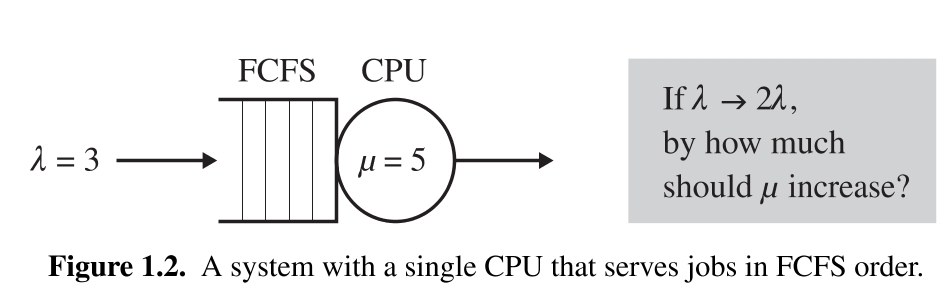
\includegraphics[scale=0.12]{images/simplequeue.jpg}
					%\caption{Sample caption.}
        		\end{center}
		    \end{figure}
		\end{itemize}
		\item \textbf{Question}: What if $\lambda  $ is doubled? 
			\begin{itemize}
			\item How the $E[T]$ changes? increases or decreases? 
			\item Can you serve customer within old	time length?
			\item If decreases, can using powerful cpu solve the problem?
			\item How much powerful CPU is necessary? ans: Less than double
			\end{itemize}
	\end{itemize}	    
    
\end{frame}

\begin{frame}
    \frametitle{Power of Queueing Theory}
    \framesubtitle{\textbf{\textit{Design Example 2}}}
	\begin{itemize}
		\item Consider the closed system of figure 
			\begin{figure}
        		\begin{center}
		            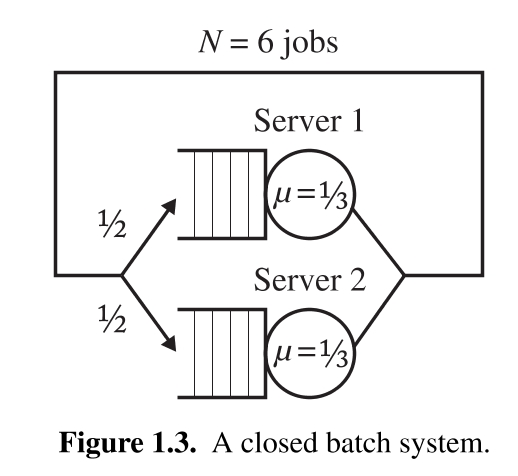
\includegraphics[scale=0.12]{images/closedbatchsystem.jpg}
					%\caption{Sample caption.}
        		\end{center}
		    \end{figure}
		\item Replace server 1 with a server that is twice as fast (the new server services jobs 						at an average rate of 2 jobs every 3 seconds).
		\begin{itemize}
			\item Does this “improvement” affect the average response time in the system?  
			\item Does it affect the throughput? 
			\item Both cases improvoment is no or negligible
		\end{itemize}
		\item If the system is converted to open system? where arrival times are independent of 						service com- pletions. 
			\begin{itemize}
				\item Absolutely possible
			\end{itemize}
	\end{itemize}	    
    
\end{frame}

\begin{frame}
    \frametitle{Power of Queueing Theory}
    \framesubtitle{\textbf{\textit{Design Example 3}}}
	\begin{itemize}
		\item one fast CPU of speed $s$,or $n$ slow CPUs each of speed $s/n$ (see Figure ). 
		\item Goal is to minimize mean response time. 
			\begin{figure}
        		\begin{center}
		            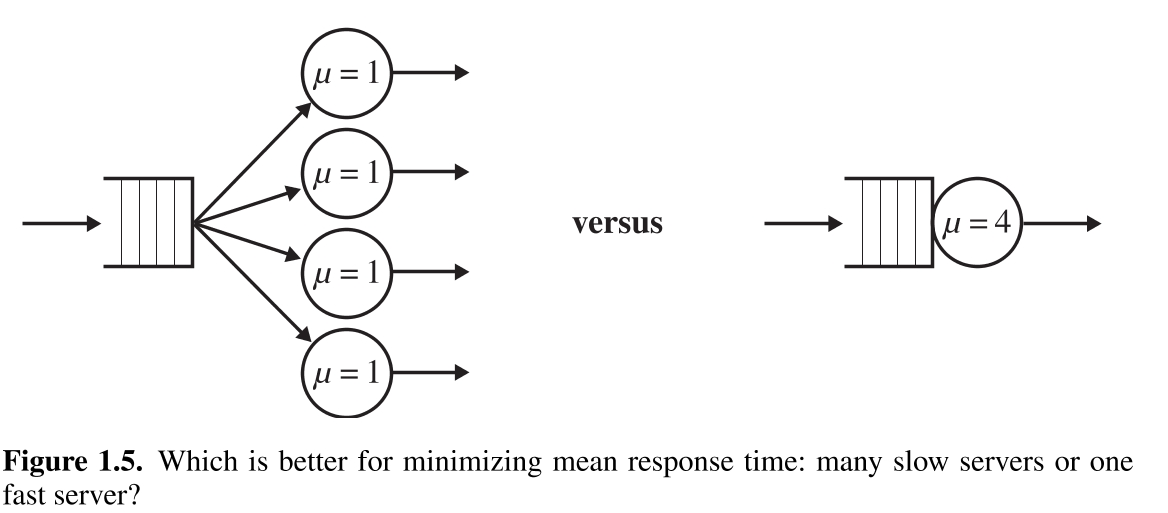
\includegraphics[scale=0.12]{images/onevsmanymachine.jpg}
					%\caption{Sample caption.}
        		\end{center}
		    \end{figure}
		\item one fast CPU of speed s,or n slow CPUs each of speed s/n (see Figure 1.5). Your goal 			is to minimize mean response time. 
		
		\begin{itemize}
			\item Choice depends on \textbf{\textit{the variability of the job size }}
		
		 
			\begin{itemize}
				\item \textbf{Question}: when job size variability is high?
					Answer:  we prefer many slow servers because we do not want short jobs getting 								stuck behind long ones.
				\item Question: Which system do you prefer when load is low?
				Answer: When load is low, not all servers will be utilized, so it seems better to 						go with one fast server.
			\end{itemize}
		\end{itemize}
	\end{itemize}	    
    
\end{frame}

\begin{frame}
    \frametitle{Power of Queueing Theory}
    \framesubtitle{\textbf{\textit{Design Example 3..cont..}}}
	\begin{itemize}
		\item If jobs are preemptible; Jobs can be stopped and restarted where they left off. 
		\item \textbf{Question} do you prefer many slow machines as compared to a single fast 					machine? 
		Answer: If your jobs are preemptible, you could always use a single fast 										machine to simulate the effect of n slow machines.  
		\item Resources can vary. CPU, GPU, MEMORY etc. 
		\item Complexity and variation grows
			
	\end{itemize}	    
    
\end{frame}

\begin{frame}
    \frametitle{Power of Queueing Theory}
    \framesubtitle{\textbf{\textit{Design Example 4}}}
	\begin{itemize}
		\item 
			\begin{figure}
        		\begin{center}
		            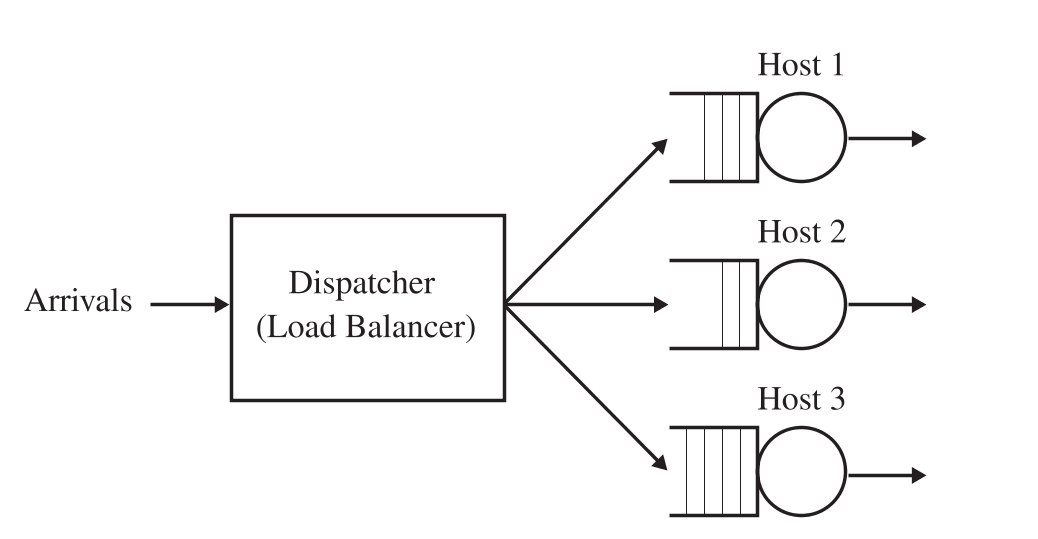
\includegraphics[scale=0.12]{images/loadbalancer.jpg}
					%\caption{Sample caption.}
        		\end{center}
		    \end{figure}
		\item Assume that all  hosts are identical (homogeneous) 
		\item all jobs only use a single resource. 
		\item  once jobs are assigned to a host, they are processed there in FCFS order and are 						non-preemptible.
		\item Which task assignment policies yields the lowest mean response time?
		\item Some options	Random, Round-Robin, Size-Interval-Task-Assignment (SITA), Central-						Queue:
		\item More possible. Answer depends on various parameters
			\begin{itemize}
			\item If job size variability is low, then the LWL policy is best. 
			\item If job size variability is high, then it is important to keep short jobs from 							getting stuck behind long ones, so a SITA-like policy, 
			\item There are many open questions with respect to task assignment policies.
			\end{itemize}
	\end{itemize}	    
    
\end{frame}

\begin{frame}
    \frametitle{Power of Queueing Theory}
    \framesubtitle{\textbf{\textit{Design Example 4}}}
	\begin{itemize}
		\item A single server. Jobs arrive according to a Poisson process. Arbitrary Job size
		\item Question : Which Scheduling policy is best w.r.t. mean response time if \textbf{non-					preemptive service orders}?
		\item Scheduling policies are: First-Come-First-Served (FCFS), Non-Preemptive Last-Come-						First-Served (LCFS), etc
		\item Ans: All are same for \textbf{non-preemptive service orders}
		\item now if \textbf{Non Preemptive-LCFS policy (PLCFS)}- Whenever a new arrival 								enters 	the system, it immediately preempts the job in service
		\item Mean resposne time depends on the variability of the job size distribution.
			\begin{itemize}
			 	\item job size distribution is at least moderately variable, then PLCFS will be a 								huge improvement.
			\end{itemize} If the job size distribution is hardly variable (basically constant), 								then PLCFS policy will be up to a factor of 2 worse.
	\end{itemize}	    
    
\end{frame}

    
\end{document}